\documentclass[tikz,border=5pt]{standalone}
\usetikzlibrary{angles,quotes,calc,arrows.meta}
\begin{document}

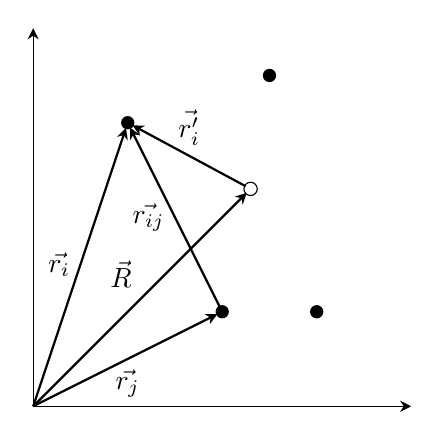
\begin{tikzpicture}[scale=1.2, 
  >={Stealth[length=4pt,width=4pt]},
  vector/.style={->,thick},
  charge/.style={circle,draw,fill=gray!20,minimum size=8pt,inner sep=0pt}
  ]
\coordinate (O) at (0,0);
\coordinate (e1) at (4,0);
\coordinate (e2) at (0,4);
\coordinate (ri) at (1,3);
\coordinate (rj) at (2,1);
\coordinate (R) at (2.3,2.3);
\coordinate (r3) at (3,1);
\coordinate (r4) at (2.5,3.5);
\fill (ri) circle (2pt);
\fill (rj) circle (2pt);
\fill (r3) circle (2pt);
\fill (r4) circle (2pt);
\filldraw[fill=white,draw=black] (R) circle (2pt);
\draw[->] (O)--(e1);
\draw[->] (O)--(e2);
\draw[thick,->,shorten >=2pt] (O)--(rj) node [midway,below] {$\vec{r_j}$};
\draw[thick,->,shorten >=2pt] (O)--(ri) node [midway,left] {$\vec{r_i}$};
\draw[thick,->,shorten >=2pt] (O)--(R) node [midway,above left] {$\vec{R}$};
\draw[thick,->,shorten >=2pt] (rj)--(ri) node [midway,left] {$\vec{r_{ij}}$};
\draw[thick,->,shorten <=2pt,shorten >=2pt] (R)--(ri) node [midway,above] {$\vec{r_{i}'}$};
\end{tikzpicture}
\end{document}